\documentclass[11pt]{article}
\usepackage[latin2]{inputenc}
\usepackage{a4wide}
\usepackage{graphicx}
\usepackage{hyperref}
\hypersetup{colorlinks=true,linkcolor=blue}
\title{Prusa Mendel Documentation}
\author{ThingDoc}

\begin{document}

\maketitle
\begin{center}

\includegraphics[width=8cm]{logo.png}
\end{center}
Prusa Mendel is machine from RepRap project. RepRap is open source 3D printer.

\newpage

\tableofcontents

\newpage

\section{Bill of Materials}
List of things you need to build the machine divided by categories.

\subsection{Rods and Bars}
\begin{itemize}
\item 1x \hyperlink{thing_idler-m8-piece}{Idler}
\end{itemize}

\subsection{Nuts\&bolts}
\begin{itemize}
\item 3x 608 skate bearing
\item 4x M4 nut
\item 3x M3 10mm screw
\item 2x M4 25mm screw
\item 1x \hyperlink{thing_hobbed-bolt}{M8 hobbed bolt}
\item 8x M3 15mm screw with HEX head
\item 2x M3 10mm screw with hex head
\item 1x M3 25mm screw
\item 1x M3 grub screw
\item 2x M3 25mm screw with HEX head
\item 12x M3 nut
\item 73x M8 washer
\item 74x M8 nut
\item 29x M3 washer
\item 1x M3 10mm screw with flat head
\item 2x M3 40mm screw
\end{itemize}

\subsection{Printed}
\begin{itemize}
\item 1x \hyperlink{thing_extruder-body}{Extruder body}
\item 8x \hyperlink{thing_bar-clamp}{Bar clamp}
\item 4x \hyperlink{thing_y-bushing}{Y bushing}
\item 2x \hyperlink{thing_frame-vertex}{Frame vertex}
\item 1x \hyperlink{thing_y-motor-bracket}{Y motor bracket}
\item 1x \hyperlink{thing_small-gear}{Small extruder gear}
\item 2x \hyperlink{thing_rod-clamp}{Rod clamp}
\item 4x \hyperlink{thing_frame-vertex-foot}{Frame vertex with foot}
\item 1x \hyperlink{thing_large-gear}{Large extruder gear}
\item 2x \hyperlink{thing_belt-clamp}{Belt clamp}
\item 1x \hyperlink{thing_idler}{Extruder Idler}
\item 1x \hyperlink{thing_z-motor-mount}{Z motor mount}
\item 1x \hyperlink{thing_x-carriage}{X carriage}
\end{itemize}

\newpage

\section{Things Overview}
List of things and their descriptions.

\hypertarget{thing_frame-triangle}{\subsection{Frame triangle}}
Two triangle parts which will later form a frame.

\hypertarget{thing_y-axis}{\subsection{Y axis}}
Assembled Y axis

\hypertarget{thing_frame-with-axes}{\subsection{Frame with axes}}
Frame with all axes mounted

\hypertarget{thing_frame-vertex}{\subsection{Frame vertex}}
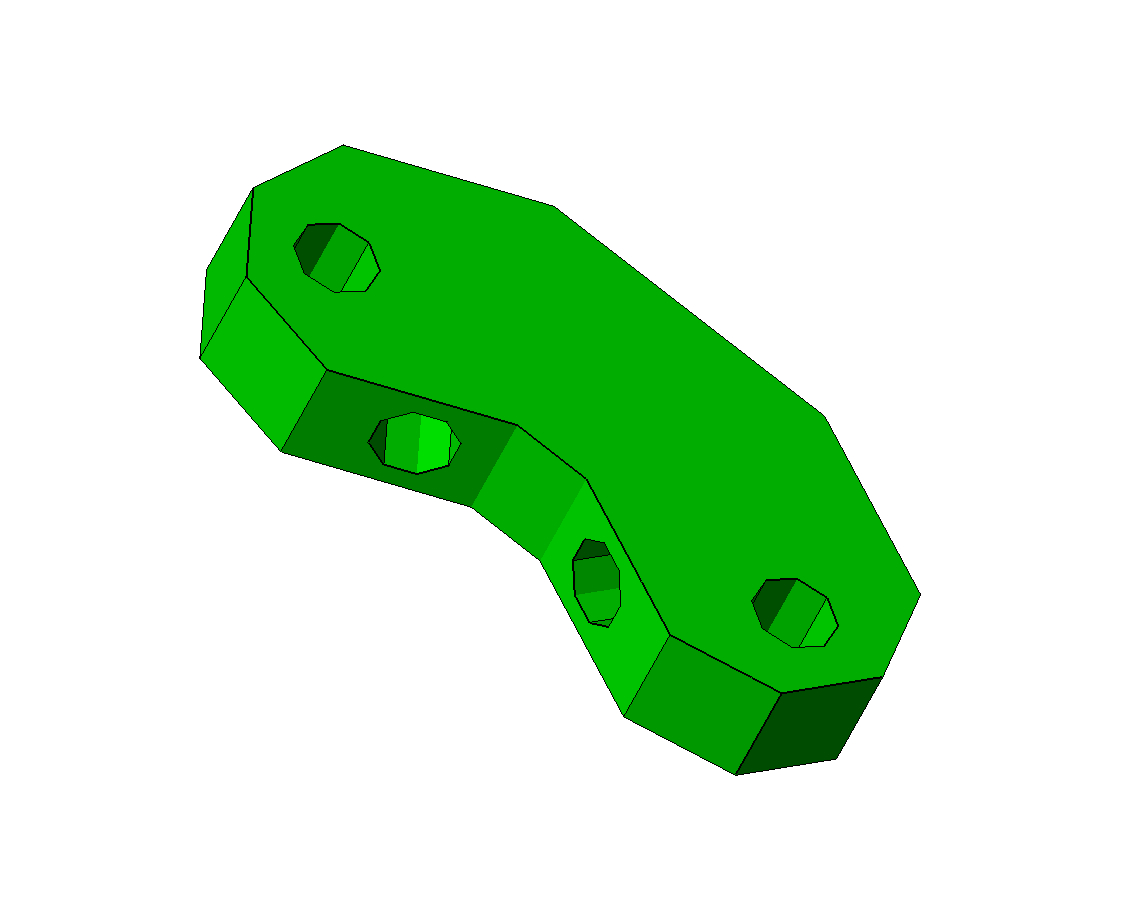
\includegraphics[width=4cm]{images/frame-vertex.jpg}

\hypertarget{thing_frame}{\subsection{Frame}}
Frame for adding all of the other parts
There is a triangle on each side of the Prusa RepRap. You will need to make two of these and then connect them together (in the next steps) to form the Prusa frame. Each side is an equilateral triangle with a frame vertex on each corner. You can use either footed or non-footed vertices to build this. (The footed ones look better, but are not critical.) The instructions assume you are using footed vertices.

\hypertarget{thing_loadtester}{\subsection{load tester}}

\hypertarget{thing_y-motor-bracket}{\subsection{Y motor bracket}}
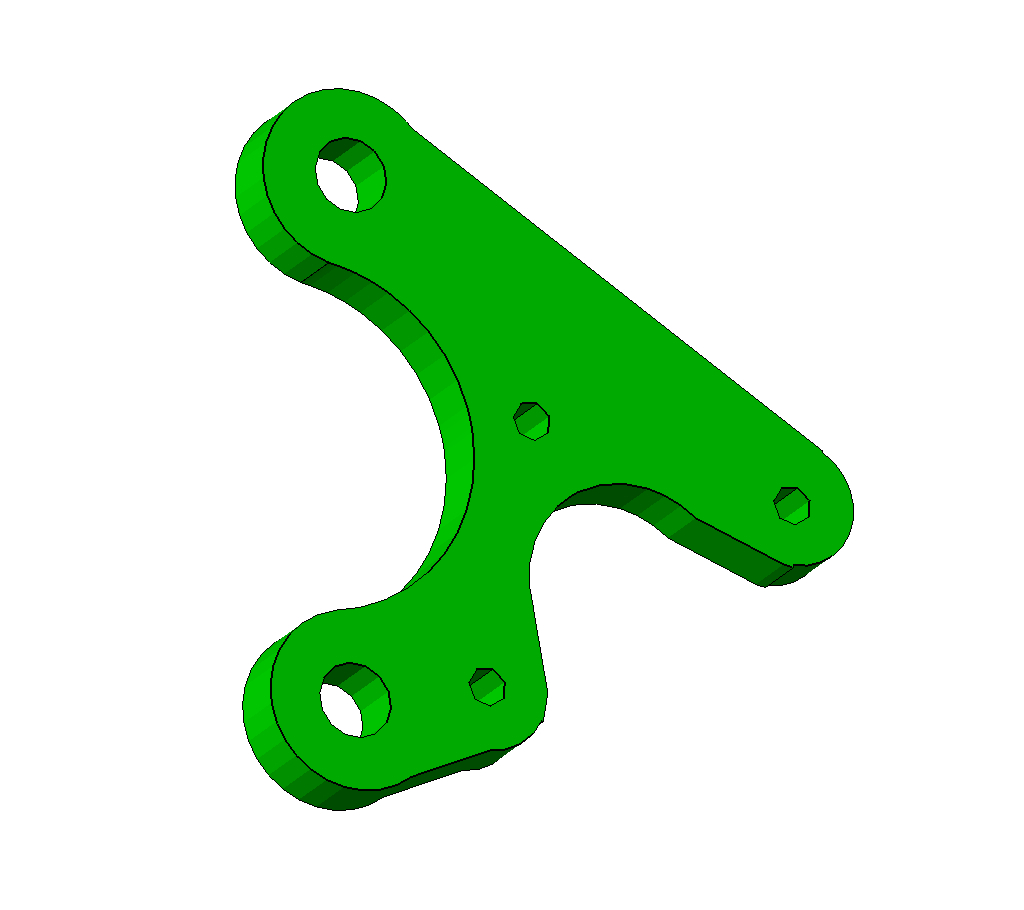
\includegraphics[width=4cm]{images/y-motor-bracket.jpg}

\hypertarget{thing_hobbed-bolt}{\subsection{M8 hobbed bolt}}

\hypertarget{thing_idler}{\subsection{Extruder Idler}}
Extruder idler

\hypertarget{thing_frame-with-y}{\subsection{Frame with Y axis}}
Frame with Y axis mounted

\hypertarget{thing_y-bushing}{\subsection{Y bushing}}

\hypertarget{thing_bar-clamp}{\subsection{Bar clamp}}
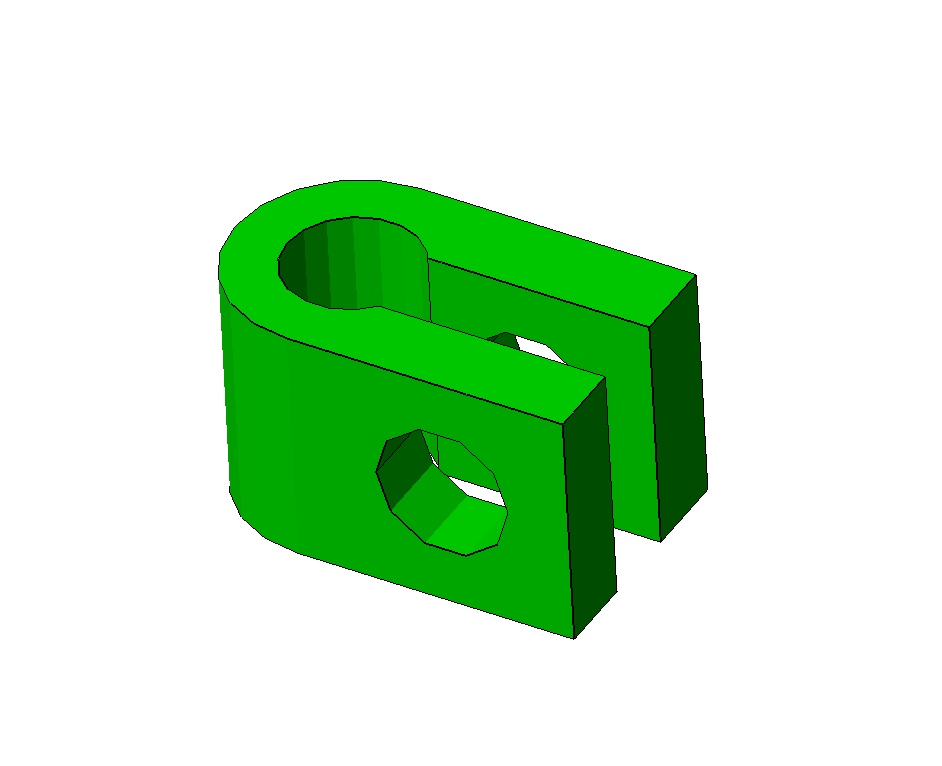
\includegraphics[width=4cm]{images/bar-clamp.jpg}

\hypertarget{thing_calibration}{\subsection{Configuration test}}

\hypertarget{thing_xz-axis}{\subsection{XZ axis}}
Assembled XZ axis

\hypertarget{thing_large-gear}{\subsection{Large extruder gear}}

\hypertarget{thing_frame-vertex-foot}{\subsection{Frame vertex with foot}}
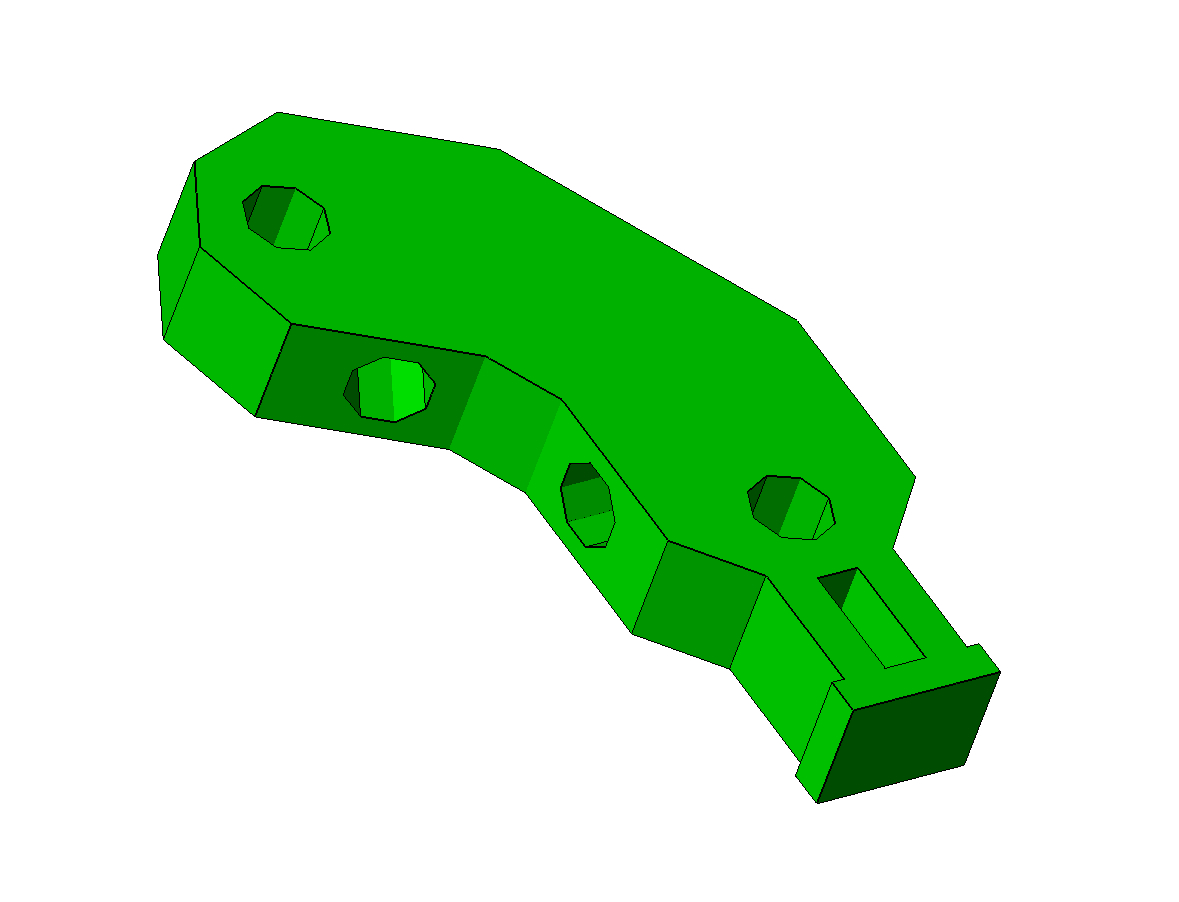
\includegraphics[width=4cm]{images/frame-vertex-foot.jpg}

\hypertarget{thing_x-end-motor}{\subsection{X end motor}}

\hypertarget{thing_extruder-body}{\subsection{Extruder body}}
Extruder body

\hypertarget{thing_small-gear}{\subsection{Small extruder gear}}

\hypertarget{thing_extruder-spring}{\subsection{Extruder spring}}
Spring used for idler on extruder.

\hypertarget{thing_printable-bushing}{\subsection{Printable Bushing}}

\hypertarget{thing_x-carriage}{\subsection{X carriage}}
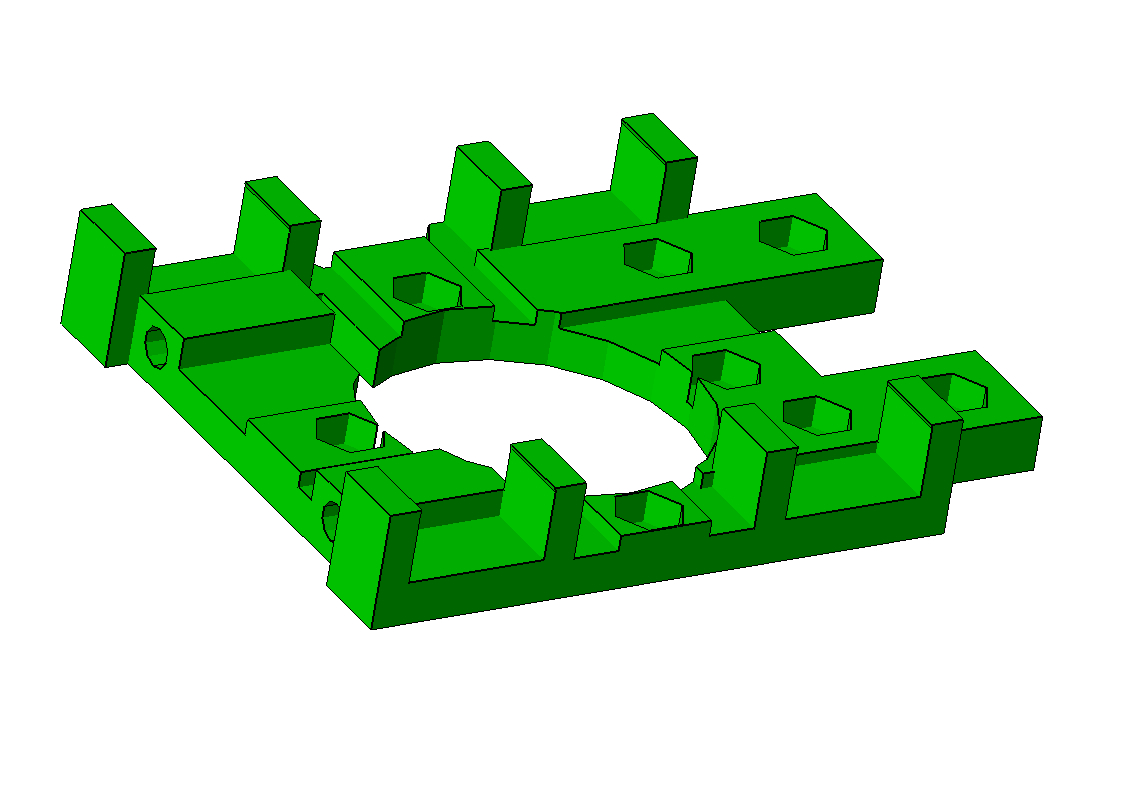
\includegraphics[width=4cm]{images/x-carriage.jpg}

\hypertarget{thing_x-end-idler}{\subsection{X end idler}}

\hypertarget{thing_rod-clamp}{\subsection{Rod clamp}}
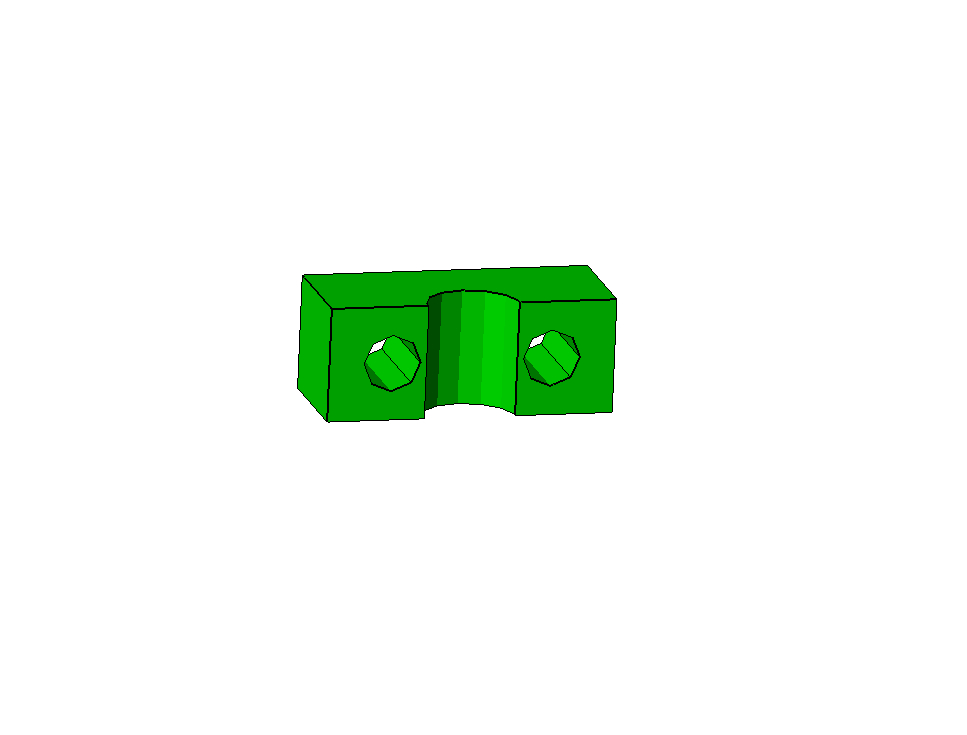
\includegraphics[width=4cm]{images/rod-clamp.jpg}

\hypertarget{thing_z-motor-mount}{\subsection{Z motor mount}}
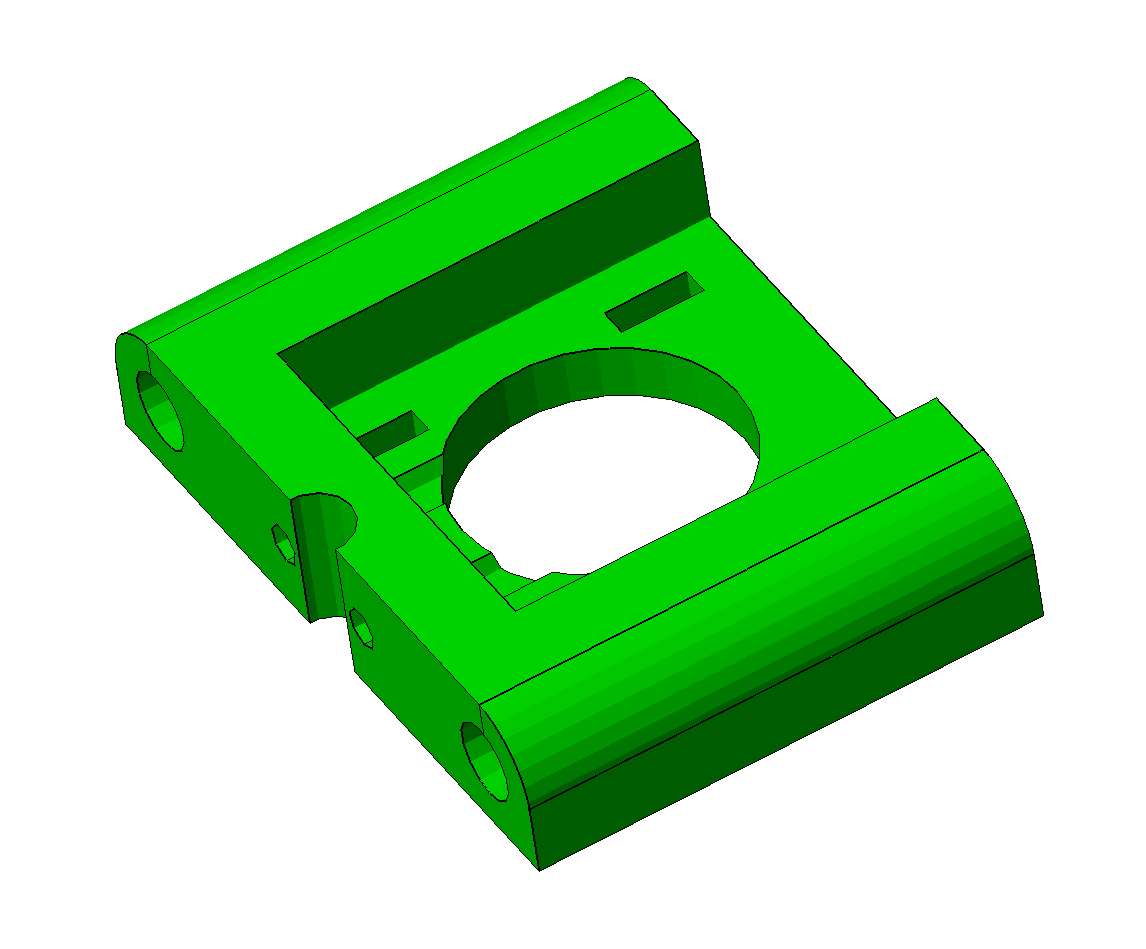
\includegraphics[width=4cm]{images/z-motor-mount.jpg}

\hypertarget{thing_endstop-holder}{\subsection{Endstop holder}}

\hypertarget{thing_bushing}{\subsection{Bushing}}

\hypertarget{thing_idler-m8-piece}{\subsection{Idler}}
Small M8 rod

\hypertarget{thing_pulley}{\subsection{Pulley}}

\hypertarget{thing_coupling}{\subsection{Coupling}}

\hypertarget{thing_carriage}{\subsection{Carriage}}
X-carriage with mounted extruder

\hypertarget{thing_belt-clamp}{\subsection{Belt clamp}}
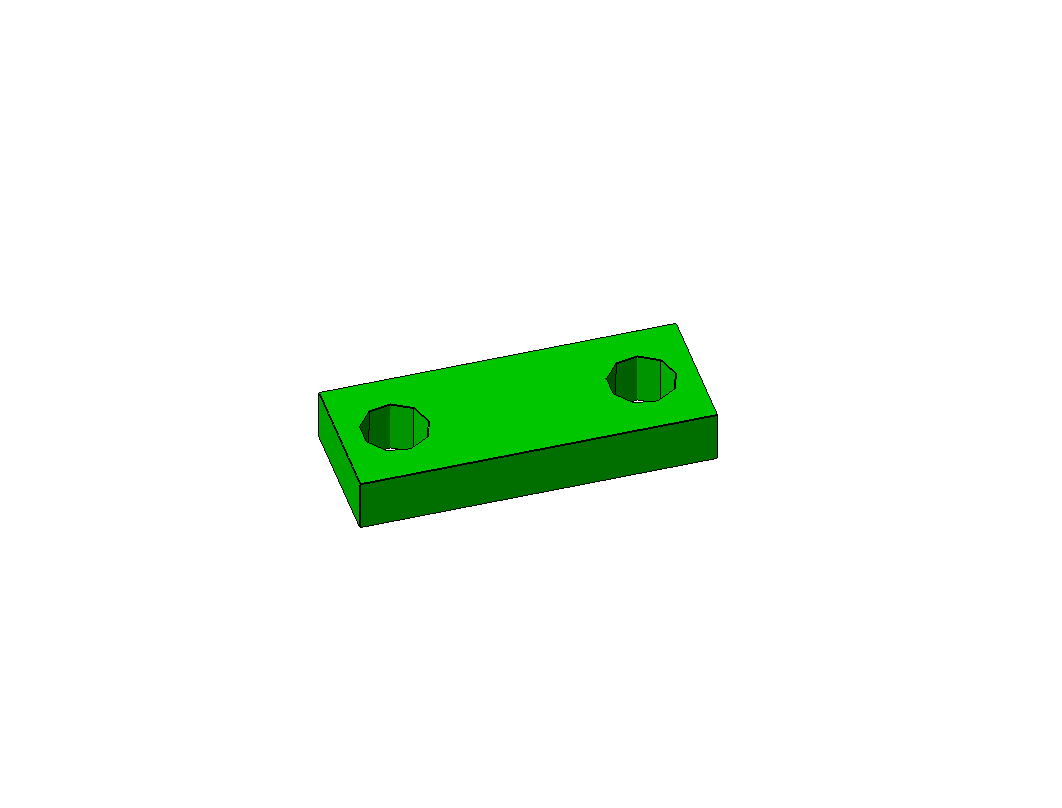
\includegraphics[width=4cm]{images/belt-clamp.jpg}

\hypertarget{thing_extruder}{\subsection{Extruder}}
Extruder

\newpage

\section{Assembly Instructions}

\subsection{Assemble Small extruder gear}
Things needed:
\begin{itemize}
\item 1x M3 nut
\item 1x M3 grub screw
\end{itemize}
Steps:
\begin{enumerate}
\item Insert nut into cavity in printed gear.
\item Tighten the grub screw a bit, just to hold in place.
\end{enumerate}

\subsection{Assemble M8 hobbed bolt}Steps:
\begin{enumerate}
\item Use thread cutting bit in electric screwdriver ...
\end{enumerate}

\subsection{Assemble Large extruder gear}
Things needed:
\begin{itemize}
\item 1x \hyperlink{thing_hobbed-bolt}{M8 hobbed bolt}
\end{itemize}
Steps:
\begin{enumerate}
\item Insert hobbed bolt into main hole.
\item Add some M8 washers from other side, later with their count you adjust position of hobbed part in filament path.
\end{enumerate}

\subsection{Assemble Extruder Idler}
Things needed:
\begin{itemize}
\item 1x 608 skate bearing
\item 1x \hyperlink{thing_idler-m8-piece}{Idler}
\end{itemize}
Steps:
\begin{enumerate}
\item Insert piece of M8 rod into bearing.
\item Insert 608 bearing with rod into printed idler part.
\end{enumerate}

\subsection{Assemble Extruder}
Things needed:
\begin{itemize}
\item 2x 608 skate bearing
\item 1x \hyperlink{thing_extruder-body}{Extruder body}
\item 3x M3 10mm screw
\item 2x M4 nut
\item 1x \hyperlink{thing_small-gear}{Small extruder gear}
\item 1x M3 25mm screw
\item 1x NEMA17 stepper motor
\item 1x \hyperlink{thing_large-gear}{Large extruder gear}
\item 8x M3 washer
\item 1x M8 washer
\item 1x \hyperlink{thing_idler}{Extruder Idler}
\item 1x M3 nut
\item 2x M3 40mm screw
\item 2x \hyperlink{thing_extruder-spring}{Extruder spring}
\item 2x M8 nut
\end{itemize}
Steps:
\begin{enumerate}
\item Take idler and insert nut into small nut-trap inside the hinge.
\item While holding the nut in place, preprare M3x25 bolt with washer and screw it into the hinge just enough to hold the nut.
\item Now take the extruder body and idler. Place idler on the hinge counterpart and compleately screw the M3x25 bolt. This will create secured hinge.
\item Place M4 nuts into their nut traps, secure them with piece of tape. We need them in place, since later they would be harder to access.
\item Prepare your NEMA17 stepper motor and three M3x10 screws with washers.
\item Hold motor on place and lightly tighten the screws. We need to adjust motor position later, no need to tighten it hard.
\item Place two skate bearings on ther position, they should snuggly fit in.
\item Insert prepared large gear into the body with mounted bearings.
\item Check if the alignment of hobbed part with the filament path. Adjust it accordingly with adding or removing M8 washers.
\item After adjusting, we need to fix the bolt in. So we place washer at the end of hobbed bolt and with two M8 nuts we will do locknut by tightening them against each other.
\item Check if large gear turns freely.
\item Prepare two M3x40 screws with sandwitch of washer-spring-washer.
\item Insert two M3 nuts into nut traps on top of drive mechanism.\\ 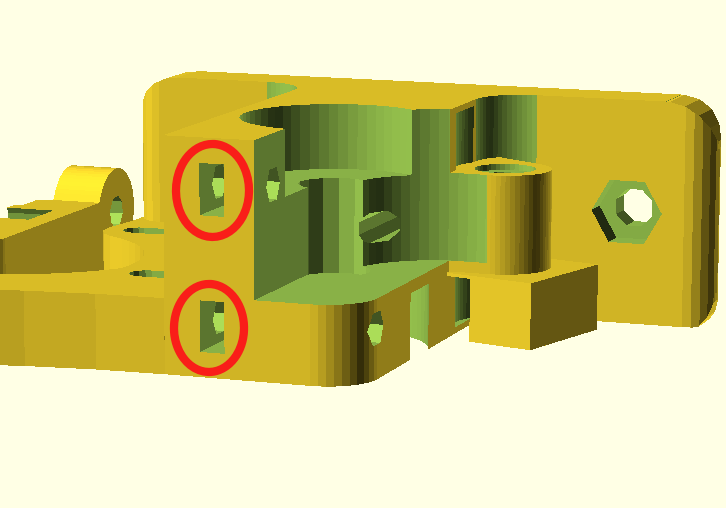
\includegraphics[width=4cm]{images/extruder/top-nut-traps.png}
\item Insert prepared screws into the holes on idler. Close the idler and tighten the screws into the trapped nuts. More you tighten those screws, more pressure will be on fillament.
\item Your extruder is done.\\ 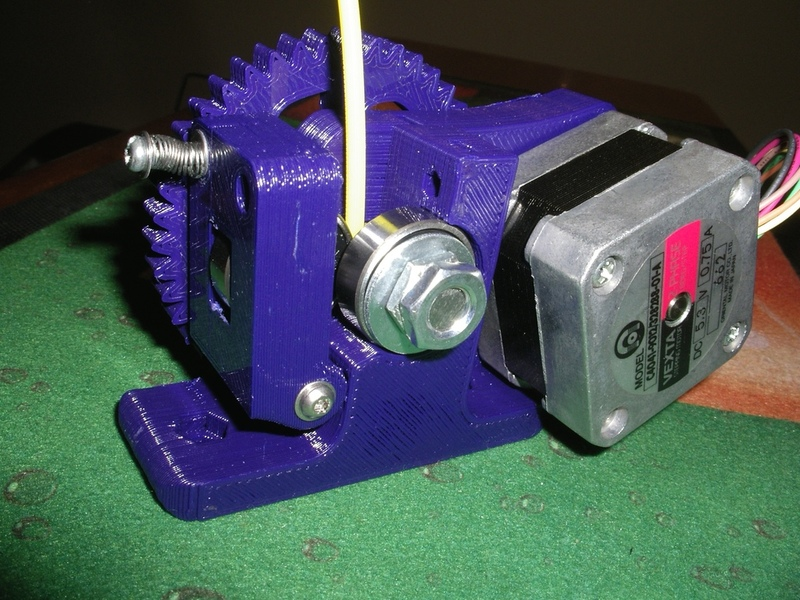
\includegraphics[width=4cm]{images/extruder/assembled.jpg}
\end{enumerate}

\subsection{Assemble Frame triangle}
Things needed:
\begin{itemize}
\item 1x \hyperlink{thing_bar-clamp}{Bar clamp}
\item 1x \hyperlink{thing_frame-vertex}{Frame vertex}
\item 2x \hyperlink{thing_frame-vertex-foot}{Frame vertex with foot}
\end{itemize}
Steps:
\begin{enumerate}
\item Take one of the 370mm threaded rods, and slip an M8 washer onto the middle of it.
\item Take the RP bar clamp (the U-shaped bit with the two holes) and slide the threaded rod through the two holes until the clamp sits next to the washer.
\item Slide another washer onto the rod from the other side.
\item Thread two M8 nuts onto either side of the clamp, until they are next to the washer, but do not tighten them yet.
\item Thread another two nuts on each side of the rod, followed by washers. See the picture for what it should look like.\\ 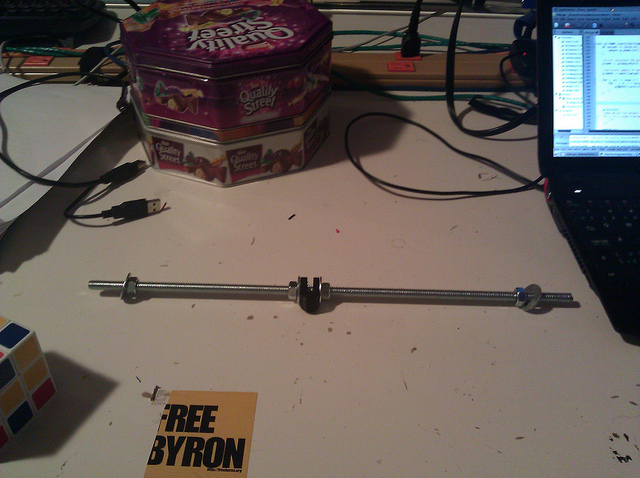
\includegraphics[width=4cm]{images/frame/threaded-rod-with-bar-clamp.jpg}
\item The bar clamp on the threaded rod.
\item Slide the rod through the wider bottom (footed) side of two vertices. Make sure the feet point in the same direction, and the bulge on the non-footed sides of the vertices point outwards.
\item Measure the distance. The distance between the two vertices should be 290mm (along the rod, equivalent is 11-13/32"). Get it approximately right now, we will check this again later. If you have a frame jig, place it between the two vertices and adjust the nuts until you can just barely fit the jig J1 between them.
\item Place another washer and nut on the other side of the vertex. Tighten, but not too much. We'll need a bit of flexibility here still.
\item Take another 370mm M8 threaded rod and place a nut followed by a washer at each end.
\item Place one end of the threaded rod into the one of the two footed frame vertices. It should be in the same plane as the first threaded rod. Fix it in place with a washer and nut. You should now have two sides of the equilateral triangle.
\item Take the third piece of threaded rod and put a nut and washer on each end. Place it in the other footed vertex and fix it in place with a washer and nut. You should now have a triangle of threaded rods with two footed vertices on two of the corners, nothing in the third corner, and a bar clamp between the two vertices.
\item Take the third vertex (non-footed) and slide it onto the threaded rods in the final corner of the triangle. Measure the lengths of the three sides to make sure they are all 290mm long (along the rod from plastic part to plastic part, equivalent is 11-13/32"). Adjust the nuts to make sure this is so. Use the frame jig J1 if you have one. Once done, place a washer and nut on each of the two rods at the top of the vertex. Tighten all the outer nuts.
\item The finished frame triangle
\item You should now have a sturdy triangle with equal-length sides, two feet on the bottom, and a bar clamp between the feet. Adjust the nuts around the bar clamp (but do not crush the bar clamp together yet) until it's approximately in the middle of the rod. Leave the nuts there loose. See the photo for what you should have at this point.
\item That's it, that's one of the triangles done. Repeat the entire procedure for the second triangle. It is identical to the first.\\ 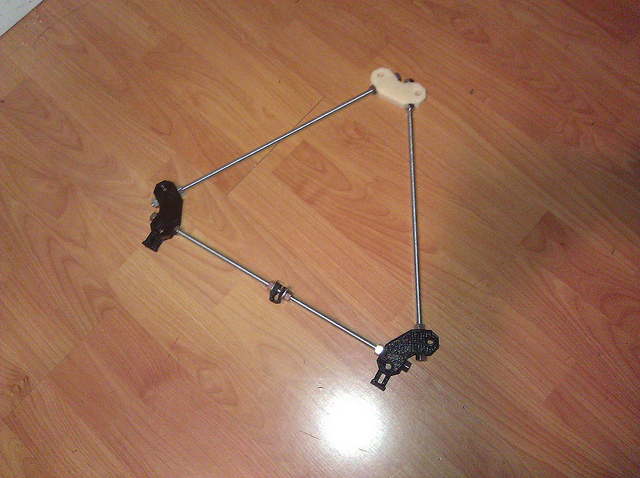
\includegraphics[width=4cm]{images/frame/finished-triangle.jpg}
\end{enumerate}

\subsection{Assemble Prusa Mendel}
Things needed:
\begin{itemize}
\item 1x \hyperlink{thing_carriage}{Carriage}
\item 1x \hyperlink{thing_frame-with-axes}{Frame with axes}
\end{itemize}
Steps:
\begin{enumerate}
\item Assembly info
\end{enumerate}

\newpage

\end{document}